\documentclass[11pt,a4paper]{article}
\usepackage[utf8]{inputenc}
\usepackage[spanish]{babel}
\usepackage{biblatex}
\usepackage{amssymb, amsmath, amsbsy}
\usepackage{graphicx}
\usepackage{makeidx}
\usepackage{color,xcolor}
\usepackage[left=2cm,right=2cm,top=2cm,bottom=2cm]{geometry}
\usepackage[linkcolor=black,colorlinks=true,urlcolor=blue]{hyperref}
\usepackage{xcolor}
\usepackage{fancyhdr}
\usepackage{float}
\usepackage{subfigure}
\renewcommand{\baselinestretch}{1.5}
\addbibresource{bib.bib}
\setlength{\parindent}{0em}
\bibliography{bib}

\begin{document}

\thispagestyle{empty}
\begin{center}

\includegraphics[width=10cm]{logo udesa.PNG}
\end{center}


	\begin{center}
	\LARGE
	Herramientas Computaciones para Investigación
\\			\vspace{1cm}
\hrule
	\vspace{0.5cm}
	\LARGE
 Tema 4 - Data Visualization
\\		
		\vspace{0.5cm}
		\hrule
				\vspace{1cm}
	\large

	\vspace{2.5cm}
	\large
		Alumnos:\\
	\large
	Elard Amaya, Francisco Guerrero
	
	
	\vspace{1.3cm}
	\normalsize	
	Profesora:\\

	\normalsize
	Amelia Gibbons
	
	\vspace{1.3cm}
	\today
	\end{center}

\clearpage
\section{Gráfico 1}

\begin{figure}[!h]
    \centering
    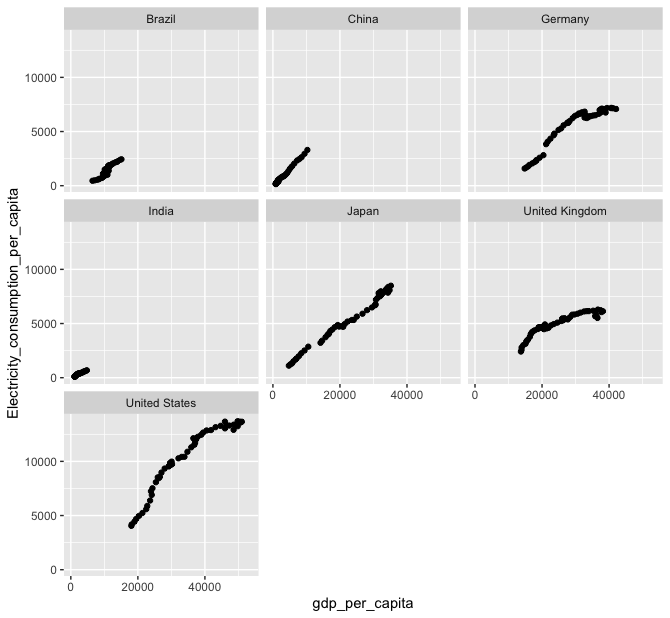
\includegraphics[width=9cm]{old/graph1.png}
\end{figure}

\begin{figure}[!h]
    \centering
    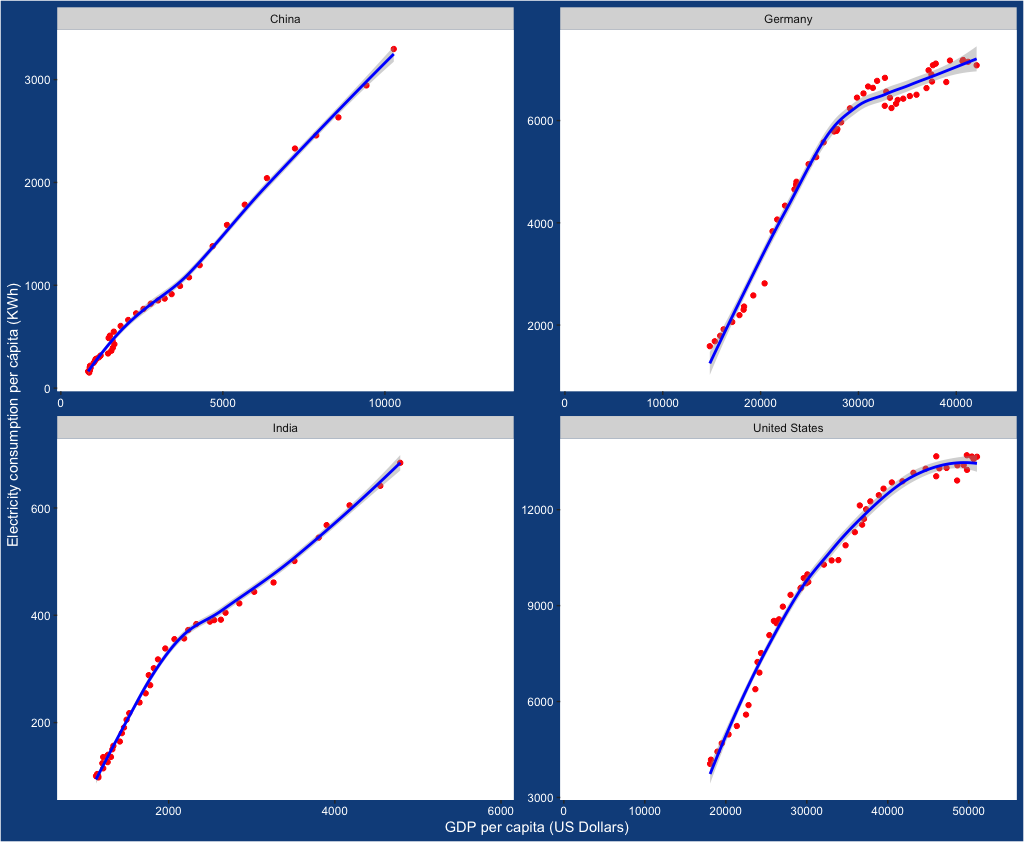
\includegraphics[width=12cm]{new/graph1.png}
\end{figure}
Con el mapa de ocurrencia de crímenes (Figura 1) buscamos identificar las zonas de mayor actividad criminal, saber si siguen algún patrón de agrupación, lo cual podría hacer estas zonas menos atrayentes para el servicio de hospedaje. Por otro lado, la tasa de aceptación de Airbnb(Figura 2) nos permite conocer cuáles son las zonas más demandadas y en consecuencia las zonas más valorizadas en el servicio de hospedajeor algunas cualidades particulares. 

\clearpage
\section{Gráfico 2}

\begin{figure}[!h]
    \centering
    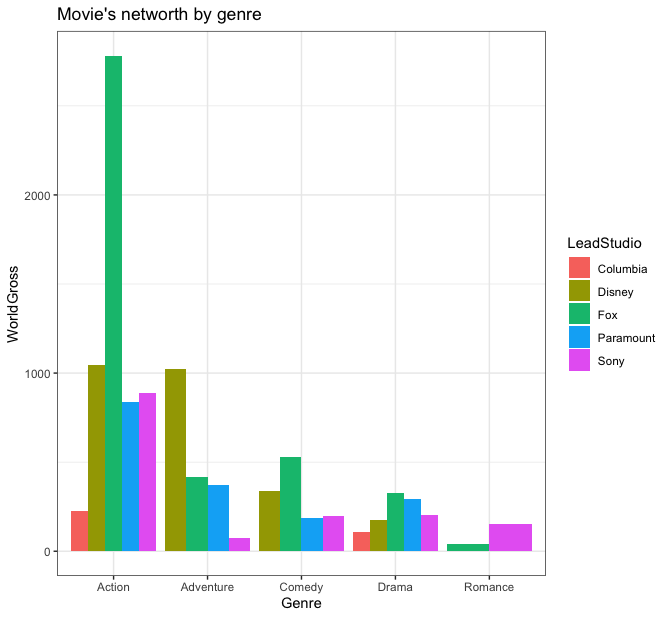
\includegraphics[width=9cm]{old/graph2.png}
\end{figure}

\begin{figure}[!h]
    \centering
    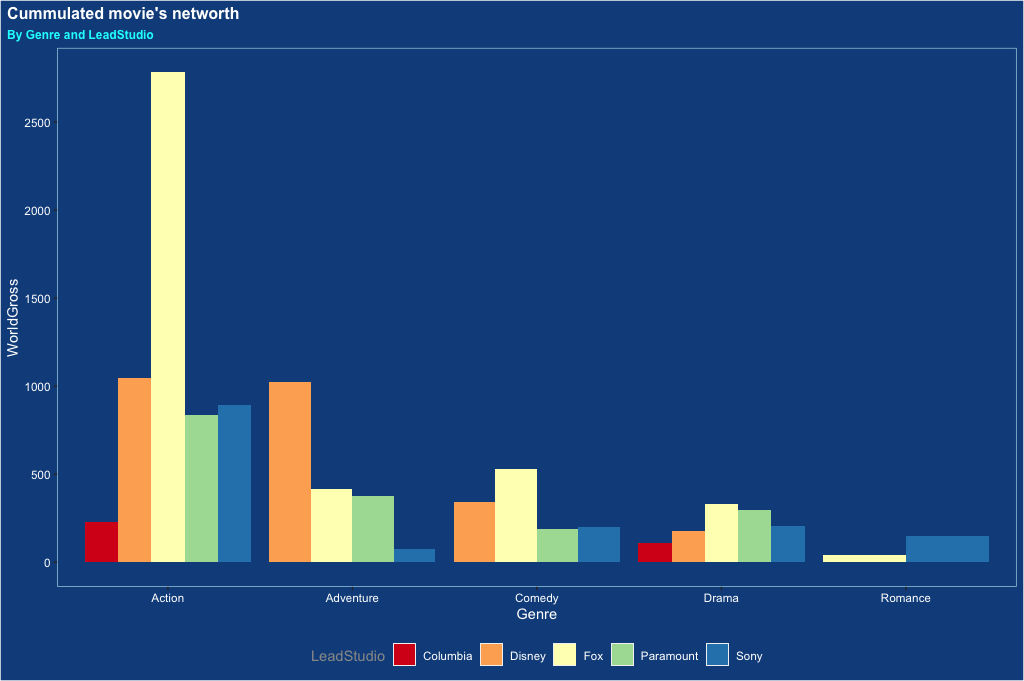
\includegraphics[width=12cm]{new/graph2.png}
\end{figure}
Con el mapa de ocurrencia de crímenes (Figura 1) buscamos identificar las zonas de mayor actividad criminal, saber si siguen algún patrón de agrupación, lo cual podría hacer estas zonas menos atrayentes para el servicio de hospedaje. Por otro lado, la tasa de aceptación de Airbnb(Figura 2) nos permite conocer cuáles son las zonas más demandadas y en consecuencia las zonas más valorizadas en el servicio de hospedajeor algunas cualidades particulares. 

\clearpage
\section{Gráfico 3}

\begin{figure}[!h]
    \centering
    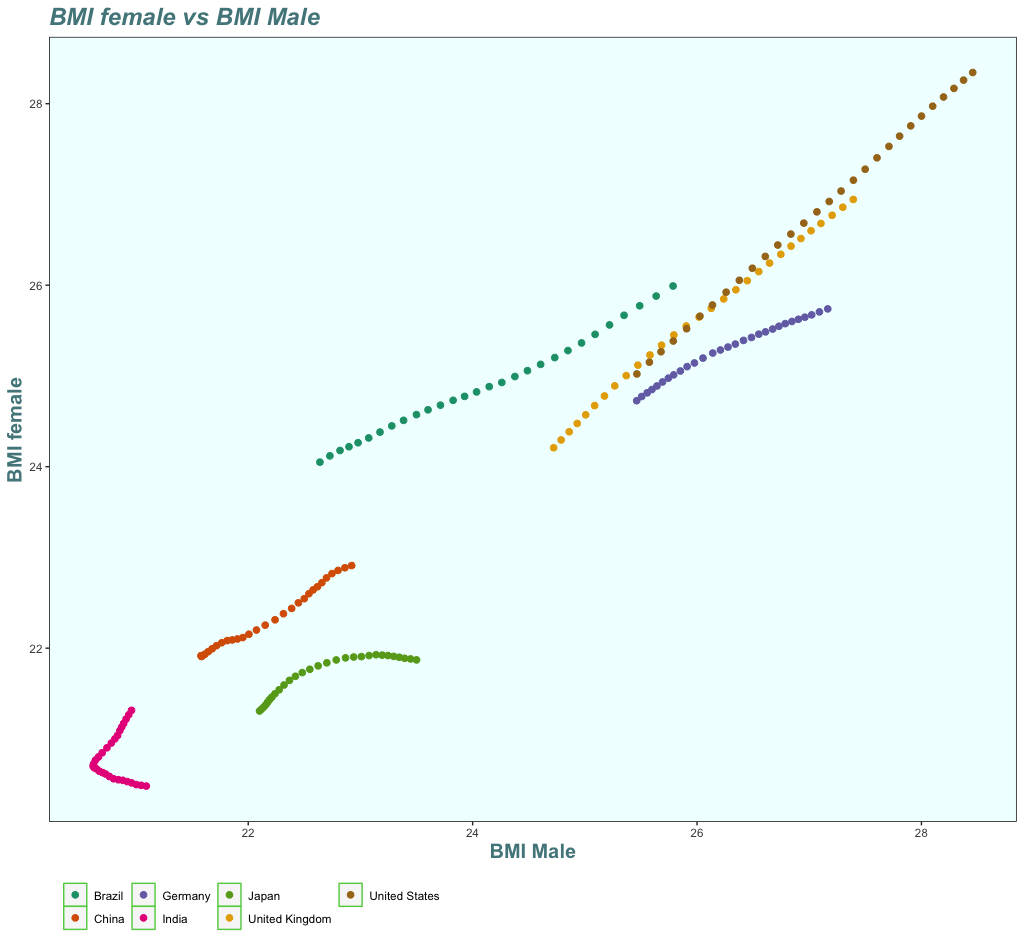
\includegraphics[width=10.5cm]{old/graph3.png}
\end{figure}

\begin{figure}[!h]
    \centering
    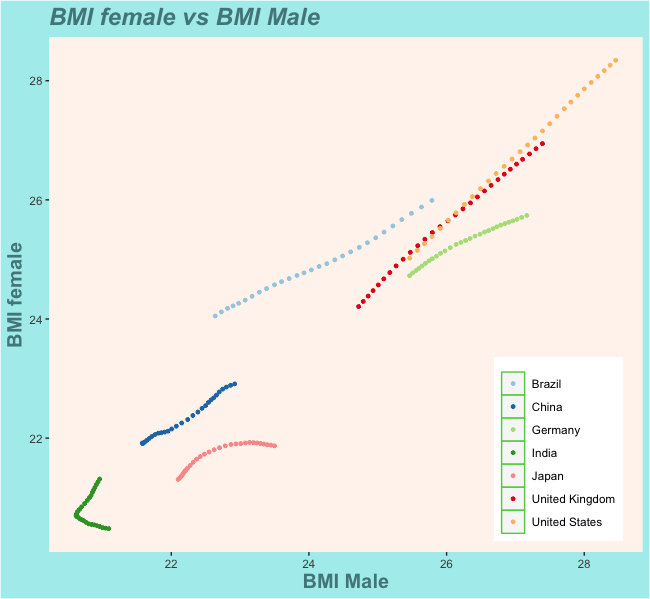
\includegraphics[width=10.5cm]{new/graph3.png}
\end{figure}


Con el mapa de ocurrencia de crímenes (Figura 1) buscamos identificar las zonas de mayor actividad criminal, saber si siguen algún patrón de agrupación, lo cual podría hacer estas zonas menos atrayentes para el servicio de hospedaje. Por otro lado, la tasa de aceptación de Airbnb(Figura 2) nos permite conocer cuáles son las zonas más demandadas y en consecuencia las zonas más valorizadas en el servicio de hospedajeor algunas cualidades particulares. 


\end{document}
